% \AtBeginSection[]{
%     \begin{frame}
%         \frametitle{}
%         \tableofcontents[currentsection]
%     \end{frame}
% }

%%%%%%%%%%%%%%%%%%%%%%%%%%%%%%%%%%%%

\section{Theoretical background: MARL \& OM}



\subsection{(G1) Multi-Agent Reinforcement Learning}

\begin{frame}{(G1) Multi-Agent Reinforcement Learning}{MARL basics}

    \begin{columns}

        \hspace{-2ex}

        \begin{column}{0.4\textwidth}

            \begin{figure}
                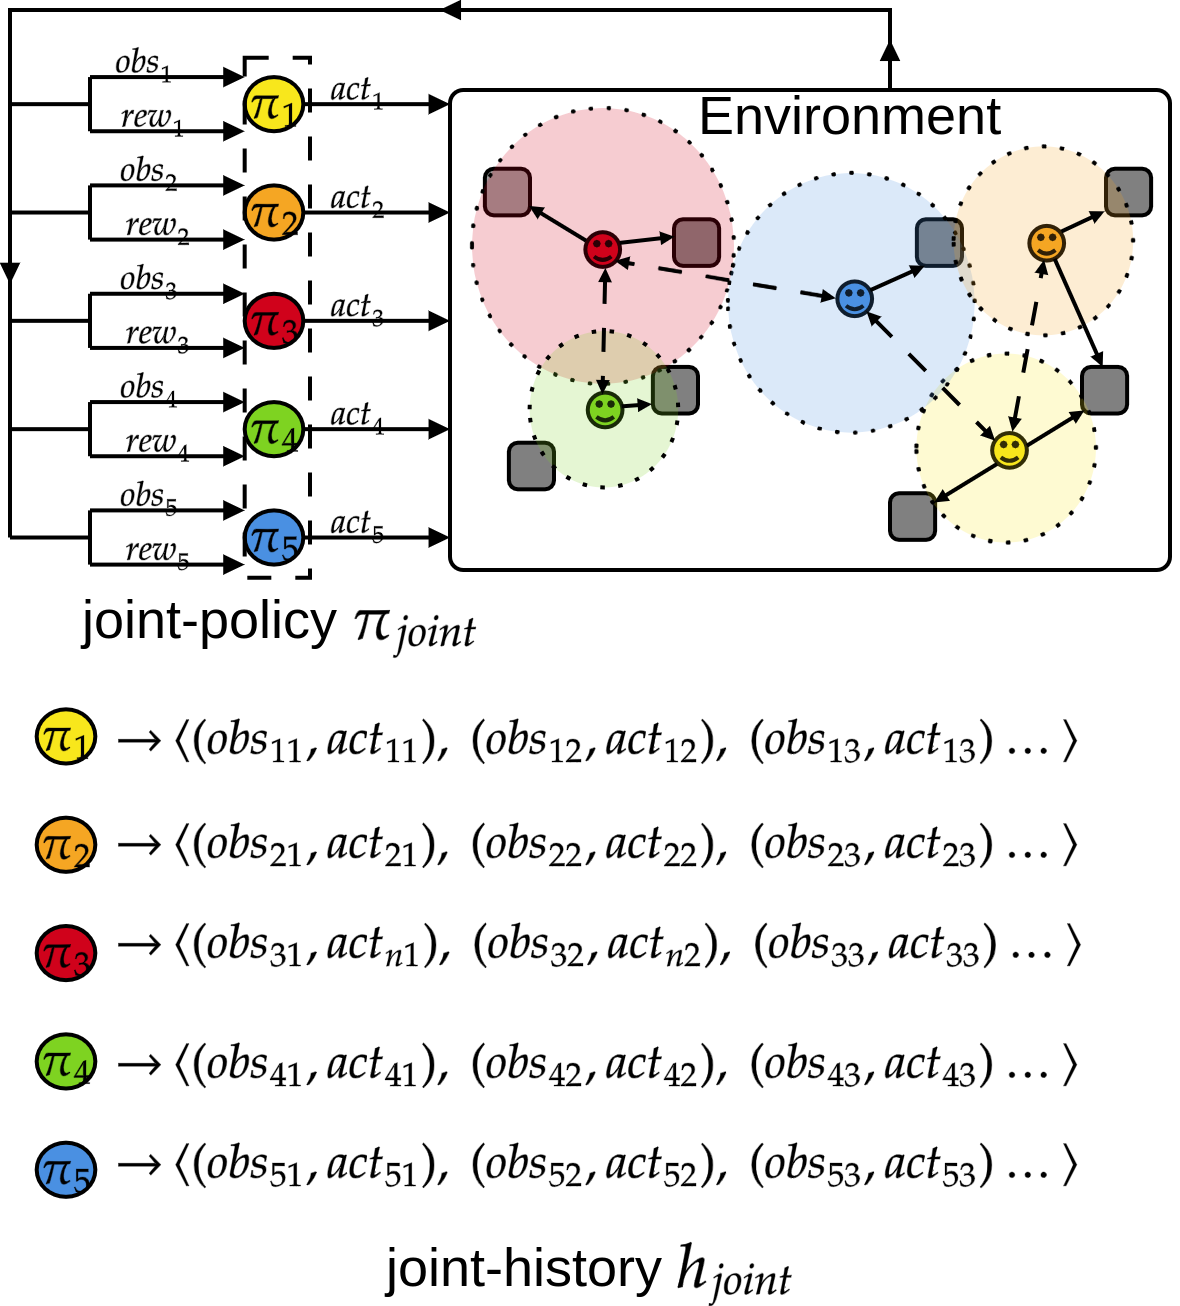
\includegraphics[width=\linewidth]{figures/marl_basics.png}
            \end{figure}

        \end{column}

        \begin{column}{0.7\textwidth}
            \vspace{-2ex}

            \begin{center}
                \begin{minipage}{0.95\linewidth}
                    \centering
                    \begin{block}{Markovian models for MARL: Dec-POMDP}
                        {\small
                            Decentralized Partially Observable Markov Decision Process (Dec-POMDP)~\cite{Oliehoek2016}
                            \begin{itemize}
                                \item considers multiple agents in a similar MAS fashion
                                \item stochastic processes for uncertainty in environmental changes including observations;
                                \item reward function is common to agents which fosters training for collaborative oriented actions~\cite{Beynier2013}
                            \end{itemize}
                        }
                        \

                        { \scriptsize

                        $(S,\{A_i\},T,R,\{\Omega_i\},O,\gamma)$ , where
                        \begin{itemize}
                            \item $S = \{s_1, ..s_{|S|}\}$: The set of the possible states;
                            \item $A_{i} = \{a_{1}^{i},..,a_{|A_{i}|}^{i}\}$: The set of the possible actions for agent $i$;
                            \item $T$ so that $T(s,a,s') = \probP{(s'|s,a)}$ : The set of conditional transition probabilities;
                            \item $R: S \times A \times S \rightarrow \mathbb{R}$: The reward function
                            \item $\Omega_{i} = \{o_{1}^{i},..,o_{|\Omega_{i}|}^{i}\}$: The set of observations for agent $ag_i$;
                            \item $O$ so that $O(s',a,o) = \probP{(o|s',a)}$ : The set of conditional observation probabilities;
                            \item $\gamma \in [0,1]$, the discount factor.
                        \end{itemize}

                        }

                    \end{block}

                \end{minipage}
            \end{center}

        \end{column}

    \end{columns}

\end{frame}

\begin{frame}{(G1) Multi-Agent Reinforcement Learning}{MARL for solving/designing}

    \begin{block}{MARL for methodological purpose in literature?}

        Effective joint-policies but \textbf{not explicitly} specified/understandable
        $\Longrightarrow$ Few related works
            {\small
                \begin{itemize}
                    \item Kazhdan et. al.~\cite{Kazhdan2020} proposed means to extract symbolic models $\rightarrow$ \textbf{not scalable};
                    \item Wang et. al.~\cite{Wang2020}: introduced a role-oriented MARL approach $\rightarrow$ \textbf{roles only};
                    \item Zheng et. al.~\cite{Zheng2018} presented a platform for MARL $\rightarrow$ \textbf{empirical tools}.
                \end{itemize}
            }
    \end{block}

    \begin{block}{Solving a Dec-POMDP}
        \begin{itemize}
            \item \textbf{solving}: finding a joint policy $\pi_{joint,i} \in \Pi_{joint}$ maximizing cumulative reward over time;
            \item \textbf{sub-optimally solving}: finding a joint policy $\pi_{joint,i} \in \Pi_{joint}$ so that expected cumulative reward over time at least at $s \in \mathbb{R}$.
        \end{itemize}
    \end{block}

    \begin{exampleblock}{Examples of MARL Algorithms}
        {\footnotesize

            \centering
            \begin{minipage}{0.5\textwidth}
                \centering
                \begin{itemize}
                    \item \textbf{Independent Learning}: IQL, IDQN
                    \item \textbf{Centralized Training, Decentralized Execution}: MADDPG, COMA, VDN
                \end{itemize}
            \end{minipage}\hfill
            \begin{minipage}{0.5\textwidth}
                \centering
                \begin{itemize}
                    \item \textbf{Cooperative MARL}: QMIX, MAPPO
                    \item \textbf{Hierarchical MARL}: Feudal Networks, Hierarchical Actor-Critic
                \end{itemize}
            \end{minipage}\hfill
        }
    \end{exampleblock}

\end{frame}



\subsection{Organizational Model}

\begin{frame}{(G2) Organizational Model}{$\mathcal{M}OISE^+$}

    \begin{figure}
        \centering
        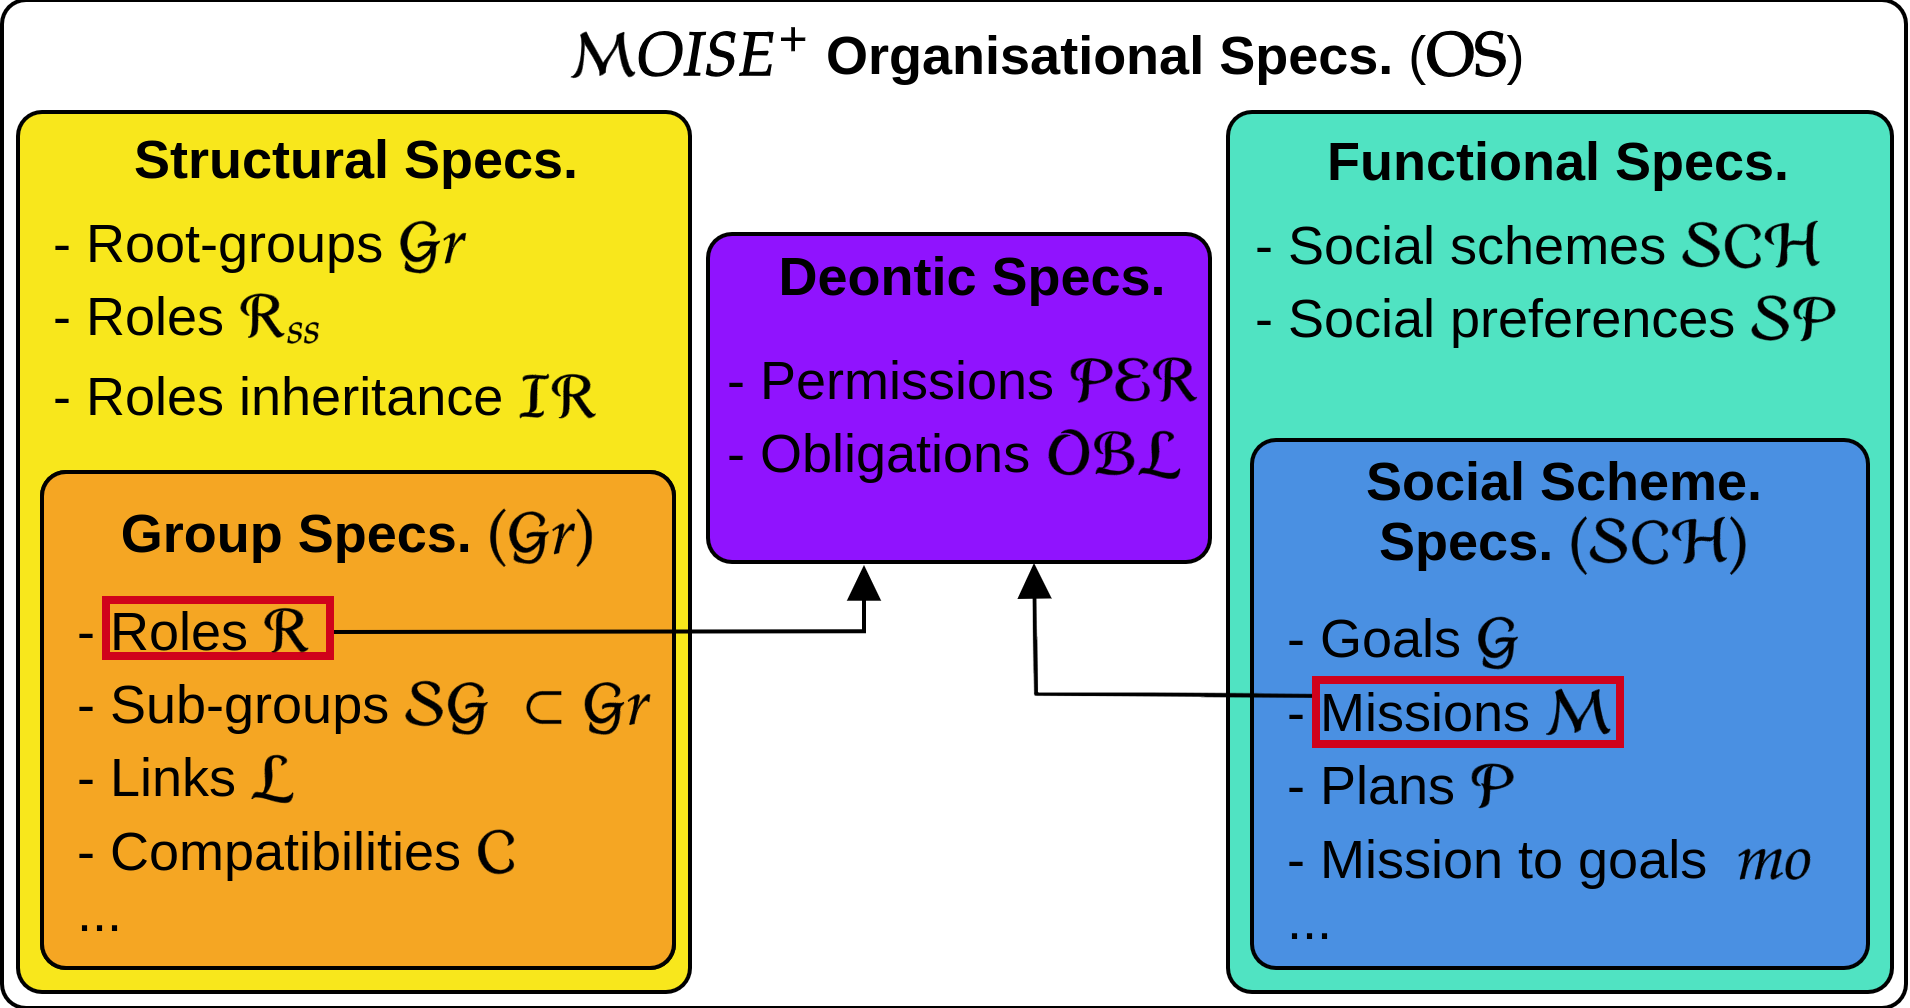
\includegraphics[width=0.75\linewidth]{figures/moise_model.png}
    \end{figure}

    \begin{spacing}{0.25}
        {\tiny Hübner, J. F., Sichman, J. S., and Boissier, O. (2002).
            A model for the structural, functional, and deontic specification of
            organizations in multiagent systems.
            In Bittencourt, G. and Ramalho, G. L., editors, Proceedings of the 16th Brazilian Symposium on Artificial Intelligence (SBIA’02), volume 2507 of LNAI, pages 118–128, Berlin. Springer.}
    \end{spacing}

\end{frame}

\begin{frame}{(G2) Organizational Model}{\textit{Soccer team example}}

    \vspace{-2.5ex}

    \begin{columns}
        \hspace{-16ex}
        \begin{column}{0.5\textwidth}
            \centering
            \begin{figure}[H]
                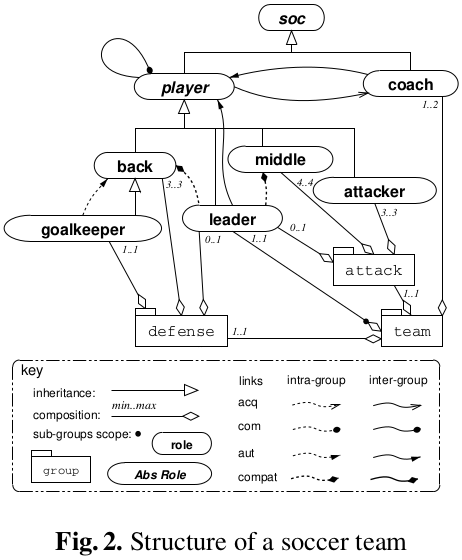
\includegraphics[width=0.7\textwidth]{figures/soccer_ss.png}
                \caption*{Structural Specifications}
            \end{figure}
        \end{column}
        \hspace{-20ex}
        \begin{column}{0.5\textwidth}
            \centering
            \begin{figure}[H]
                \centering
                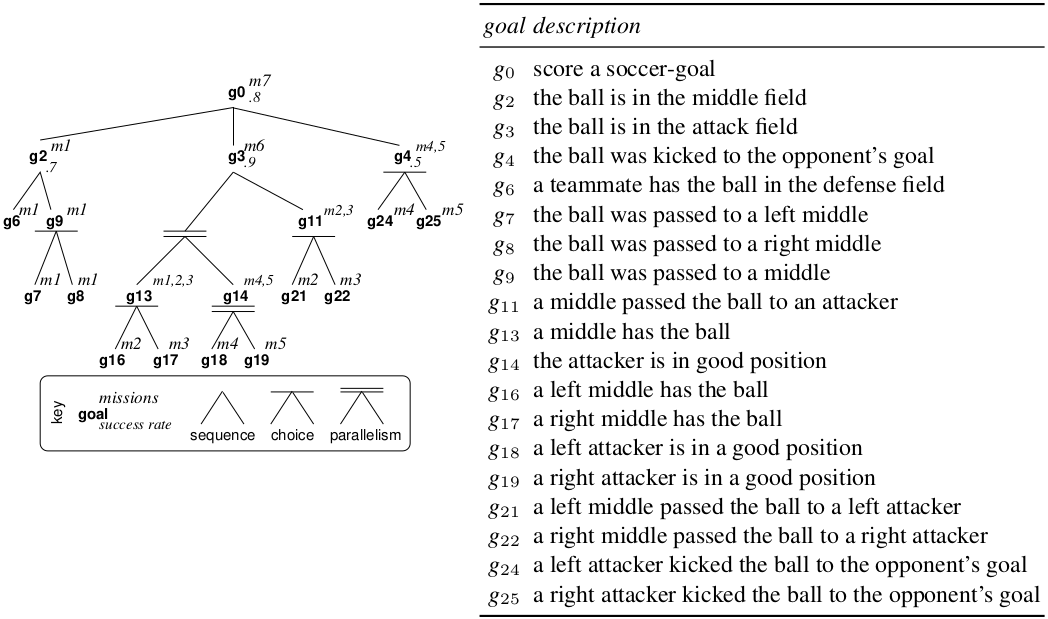
\includegraphics[width=1.2\textwidth]{figures/soccer_fs.png}
                \caption*{Functional Specifications}
            \end{figure}
        \end{column}
    \end{columns}

    % \begin{minipage}{0.5\textwidth}
    %     \centering

    % \end{minipage}\hfill
    % %
    % \begin{minipage}{0.5\textwidth}
    %     \centering

    % \end{minipage}\hfill

    \ \\

    \begin{minipage}{\textwidth}
        \centering
        \begin{figure}[H]
            \centering
            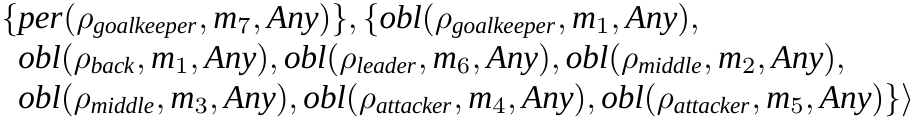
\includegraphics[width=0.4\linewidth]{figures/soccer_ds.png}
            \caption*{Deontic Specifications}
        \end{figure}
    \end{minipage}

    % \begin{figure}
    %     \centering
    %     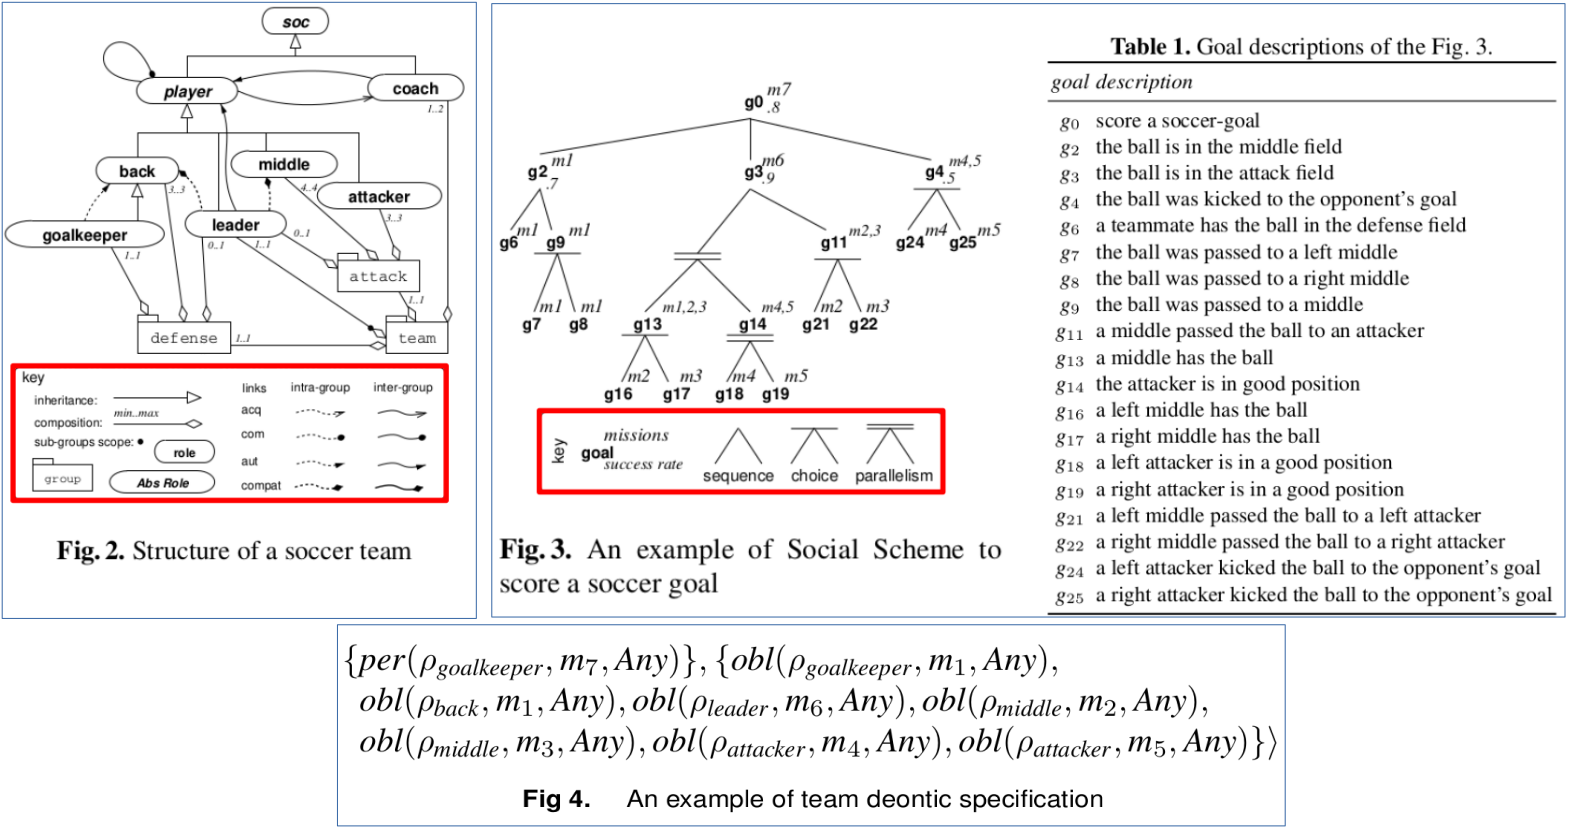
\includegraphics[width=\linewidth]{figures/soccer_os.png}
    % \end{figure}

\end{frame}
